% Created 2023-01-20 vie 12:10
% Intended LaTeX compiler: pdflatex
\documentclass[aspectratio=169, usenames,svgnames,dvipsnames]{beamer}
\usepackage[utf8]{inputenc}
\usepackage[T1]{fontenc}
\usepackage{graphicx}
\usepackage{longtable}
\usepackage{wrapfig}
\usepackage{rotating}
\usepackage[normalem]{ulem}
\usepackage{amsmath}
\usepackage{amssymb}
\usepackage{capt-of}
\usepackage{hyperref}
\usepackage{color}
\usepackage{listings}
\usepackage{mathpazo}
\usepackage{gensymb}
\usepackage{amsmath}
\usepackage{diffcoeff}
\usepackage{steinmetz}
\usepackage{mathtools}
\usepackage{fancyvrb}
\DefineVerbatimEnvironment{verbatim}{Verbatim}{fontsize=\tiny, formatcom = {\color{black!70}}}
\bibliographystyle{plain}
\usepackage{siunitx}
\sisetup{output-decimal-marker={,}}
\DeclareSIUnit{\watthour}{Wh}
\DeclareSIUnit{\wattpeak}{Wp}
\DeclareSIUnit{\watthour}{Wh}
\DeclareSIUnit{\amperehour}{Ah}
\usepackage{steinmetz}
\hypersetup{colorlinks=true, linkcolor=Blue, urlcolor=Blue}
\renewcommand{\thefootnote}{\fnsymbol{footnote}}
\parskip=5pt
\usetheme{Boadilla}
\usecolortheme{rose}
\usefonttheme{serif}
\author{\href{https://oscarperpinan.github.io}{Oscar Perpiñán Lamigueiro}}
\date{}
\title{Inversores para Centrales Fotovoltaicas}
\subtitle{Energía Solar Fotovoltaica}
\institute[UPM]{Universidad Politécnica de Madrid}
\setbeamercolor{alerted text}{fg=blue!50!black} \setbeamerfont{alerted text}{series=\bfseries}
\AtBeginSubsection[]{\begin{frame}[plain]\tableofcontents[currentsubsection,sectionstyle=show/hide,subsectionstyle=show/shaded/hide]\end{frame}}
\AtBeginSection[]{\begin{frame}[plain]\tableofcontents[currentsection,hideallsubsections]\end{frame}}
\beamertemplatenavigationsymbolsempty
\setbeamertemplate{footline}[frame number]
\setbeamertemplate{itemize items}[triangle]
\setbeamertemplate{enumerate items}[circle]
\setbeamertemplate{section in toc}[circle]
\setbeamertemplate{subsection in toc}[circle]
\hypersetup{
 pdfauthor={\href{https://oscarperpinan.github.io}{Oscar Perpiñán Lamigueiro}},
 pdftitle={Inversores para Centrales Fotovoltaicas},
 pdfkeywords={},
 pdfsubject={},
 pdfcreator={Emacs 28.2 (Org mode 9.6)}, 
 pdflang={Spanish}}
\begin{document}

\maketitle


\section{Conceptos Generales}
\label{sec:org8712ec6}
\begin{frame}[label={sec:orgbe2d917}]{Acoplamiento a la red}
\begin{block}{}
La potencia suministrada por un generador fotovoltaico iluminado es de
tensión continua, que debe ser adecuadamente acondicionada para permitir
el funcionamiento correcto de las cargas conectadas en un sistema
autónomo o el acoplamiento a la red eléctrica en el caso de sistemas de
conexión a red.
\end{block}
\end{frame}

\begin{frame}[label={sec:org5f9ade9}]{Definición}
\begin{itemize}
\item El equipo de acondicionamiento de potencia, denominado inversor DC/AC, realiza la \alert{conversión de continua a alterna cumpliendo con  determinados requisitos} de tensión eficaz, frecuencia, distorsión armónica de las ondas de tensión y corriente, rendimiento instantáneo y medio, seguridad eléctrica, etc.

\item Funciona como fuente de corriente autoconmutada y sincronizada con la red.
\end{itemize}
\end{frame}

\begin{frame}[label={sec:org22b456a}]{Tipos de Inversores}
A grandes rasgos, los inversores pueden agruparse en tres categorías:

\begin{itemize}
\item \alert{Inversor central}: un único inversor dedicado a todo el generador (o
a un conjunto de ramas)

\item \alert{Inversor orientado a rama} (\emph{string-inverter}): un inversor dedicado
a una rama del generador.

\item \alert{Módulo-AC}: un inversor dedicado a un módulo del generador.
\end{itemize}
\end{frame}

\begin{frame}[label={sec:org6800c58}]{Inversores Centrales}
\begin{itemize}
\item Los \alert{inversores centrales} son recomendables para instalaciones de
medio o gran tamaño. Permiten reducir costes (de adquisición,
instalación y mantenimiento) y aumentar fiabilidad y eficiencia.

\item \alert{La potencia del inversor debe estar en consonancia con la potencia
del generador} (una planta de 1 MWp debiera contar con 10 inversores
de 100 kW o 4 de 250 kW, pero no con 200 de 5 kW).
\end{itemize}
\end{frame}

\section{Características básicas}
\label{sec:org06469e5}
\begin{frame}[label={sec:orgbbd667c}]{Potencia y ventana MPP}
\begin{itemize}
\item \alert{Potencia nominal y máxima}, siendo ésta un porcentaje de sobrecarga
que el equipo es capaz de soportar durante un determinado período de
tiempo (indicado por el fabricante).

\item \alert{Ventana de búsqueda del Punto de Máxima Potencia} (MPP en siglas
inglesas): es el rango de tensiones en las que el inversor aplica un
algoritmo de búsqueda del MPP del generador fotovoltaico.
\end{itemize}
\end{frame}

\begin{frame}[label={sec:org337eebe}]{Tensiones}
\begin{itemize}
\item \alert{Tensión máxima de entrada}: es la máxima tensión que el inversor
puede aguantar sin sufrir una avería.

\item \alert{Tensión nominal de salida}: es la tensión de red a la que se puede
conectar el inversor (habitualmente 230 Vac para equipos monofásicos
y 400 Vac para equipos trifásicos).

\item \alert{Umbral de arranque}: según las unidades en las que se expresa, puede
indicar la radiación solar incidente en el generador
(\(\si{\watt\per\meter\squared}\)) o la potencia de entrada (W)
necesaria para que el inversor comience el proceso de conversión.
\end{itemize}
\end{frame}

\begin{frame}[label={sec:org145f8a4}]{Eficiencia}
\begin{itemize}
\item \alert{Eficiencia del inversor}, \(\eta_{inv} = P_{ac} / P_{dc}\)

\item Esta relación puede describirse con una función basada en tres
coeficientes y la normalización de la potencia de salida,
\(p_{o}=P_{ac}/P_{inv}\):
$$\eta_{inv}=\frac{p_{o}}{p_{o}+k_{0}^{o}+k_{1}^{o}p_{o}+k_{2}^{o}p_{o}^{2}}$$

\item \alert{Eficiencia máxima}: máximo valor que toma la relación entre
potencia de salida y potencia de entrada. En inversores de calidad
la eficiencia es estable en un amplio rango de funcionamiento del
equipo y de un valor cercano a la eficiencia máxima.
\end{itemize}
\end{frame}


\begin{frame}[label={sec:org9d8624f}]{Ejemplo de curva de eficiencia}
\begin{columns}
\begin{column}{0.8\columnwidth}
\begin{center}
\includegraphics[height=0.9\textheight]{../figs/CurvaInversor.pdf}
\end{center}
\end{column}


\begin{column}{0.2\columnwidth}
\(k_{0}^{o}=0.01\)

\(k_{1}^{o}=0.025\)

\(k_{2}^{o}=0.05\)
\end{column}
\end{columns}
\end{frame}

\begin{frame}[label={sec:org3ff2b49}]{Rendimiento}
\begin{itemize}
\item \alert{Rendimiento}: es la relación entre la energía entregada por
un inversor que recibe una energía producida por un generador
fotovoltaico funcionando en unas determinadas condiciones de radiación.

\item \alert{Rendimiento europeo}: condiciones de radiación características del
clima de la zona centroeuropea.
\[
  \eta_{euro} = 0.03 \cdot \eta_{5\%}  +  0.06 \cdot \eta_{10\%}  +  0.13 \cdot \eta_{20\%}  +  0.1 \cdot \eta_{30\%}  +  0.48 \cdot \eta_{50\%}  +  0.2 \cdot \eta_{100\%}
\]
\item \alert{Rendimiento CEC}: condiciones de radiación características del clima de
California.
\[
  \eta_{CEC} = 0.04 \cdot \eta_{10\%}  +  0.05 \cdot \eta_{20\%}  +  0.12 \cdot \eta_{30\%}  +  0.21 \cdot \eta_{50\%} + 0.53 \cdot \eta_{75\%}  +  0.05 \cdot \eta_{100\%}
\]
\end{itemize}
\end{frame}

\begin{frame}[label={sec:org26013d1}]{Distorsión armónica}
Cuando una señal sinusoidal atraviesa un circuito no lineal (diodos, transistores) aparecen señales (armónicos) de frecuencias múltiplo de la original (fundamental).


\begin{center}
\includegraphics[height=0.6\textheight]{../figs/DistorsionArmonica.pdf}
\end{center}
\end{frame}


\begin{frame}[label={sec:org434dd17}]{Distorsión armónica}
La distorsión armónica total (THD) es la relación entre la potencia de los armónicos superiores al fundamental (\(n > 2\)) y la potencia del fundamental.

\[
  THD_I = \frac{1}{I_1} \cdot \sqrt{\sum_{n = 2}^\infty I_n^2} 
\]

Los inversores de conexión a red suministran una señal de calidad, con \(THD < 3\%\) o inferiores.
\end{frame}

\section{Composición}
\label{sec:orgac31ce9}
\begin{frame}[label={sec:org43f70be}]{Entrada}
\begin{center}
\includegraphics[width=.9\linewidth]{../figs/InversorPV.pdf}
\end{center}

\begin{itemize}
\item \alert{Filtro de entrada}: atenúa el rizado que produce la conmutación en
la corriente de entrada

\item \alert{Convertidor DC/DC}: adecúa (eleva o reduce) la tensión de salida del
generador a la tensión necesaria para el puente de conmutación. Puede
realizar las funciones de búsqueda del punto de máxima potencia.
\end{itemize}
\end{frame}

\begin{frame}[label={sec:org9651f9f}]{Puente y salida}
\begin{center}
\includegraphics[width=.9\linewidth]{../figs/InversorPV.pdf}
\end{center}

\begin{itemize}
\item \alert{Puente inversor}: realiza el troceado de la señal continua para
convertirla en alterna

\item \alert{Filtro de salida}: elimina o atenúa los armónicos no deseados

\item \alert{Transformador}: adecua el valor de tensión de salida del puente al
de la red y proporciona aislamiento galvánico entre la parte DC y
AC.
\end{itemize}
\end{frame}

\begin{frame}[label={sec:org54580f6}]{Control}
\begin{center}
\includegraphics[width=.9\linewidth]{../figs/InversorPV.pdf}
\end{center}

\begin{itemize}
\item \alert{Control}: realiza la supervisión de la entrada y salida del
convertidor DC/DC y del puente inversor y entrega las consignas
correspondientes para localizar y seguir el MPP del generador, y para
obtener una señal sinusoidal con bajo contenido en armónicos en la
salida del inversor.
\end{itemize}
\end{frame}

\section{Funcionamiento}
\label{sec:orgaa5b33a}

\begin{frame}[label={sec:orgafe8cab}]{Modulación SPWM (monofásico)}
\begin{center}
\includegraphics[height=0.9\textheight]{../figs/SPWMMonofasico.pdf}
\end{center}
\end{frame}

\begin{frame}[label={sec:org9153e76}]{Modulación SPWM (trifásico)}
\begin{center}
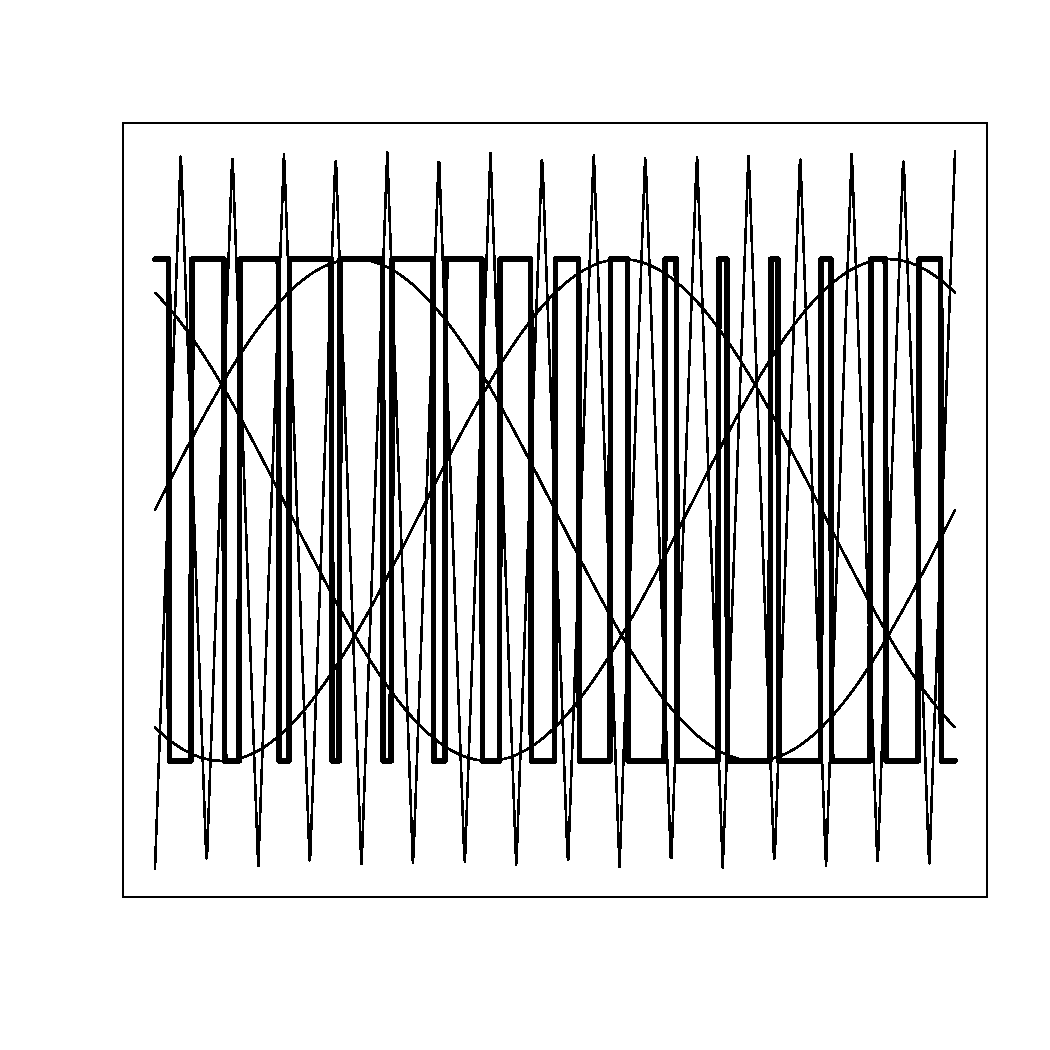
\includegraphics[height=0.9\textheight]{../figs/SPWMTrifasico.pdf}
\end{center}
\end{frame}

\begin{frame}[label={sec:org45e39c5}]{Modulación SPWM (trifásico)}
\begin{center}
\includegraphics[height=0.9\textheight]{../figs/SPWMTrifasico_shaded.pdf}
\end{center}
\end{frame}

\begin{frame}[label={sec:orgdf65389}]{Busqueda del Punto de Máxima Potencia}
\begin{center}
\includegraphics[height=0.6\textheight]{../figs/CurvaIV_Ta20_G800.pdf}
\end{center}

$$\begin{cases}
      \frac{dP}{dV}>0 & 0<V<V_{mpp}\\
      \frac{dP}{dV}=0 & V=V_{mpp}\\
      \frac{dP}{dV}<0 & V_{mpp}<V<V_{oc}\end{cases}$$
\end{frame}

\begin{frame}[label={sec:org3d5065f}]{Busqueda del Punto de Máxima Potencia}
\begin{center}
\includegraphics[height=0.6\textheight]{../figs/CurvaIV_Ta20_G800.pdf}
\end{center}

$$\begin{cases}
      \frac{dI}{dV}>-\frac{I}{V} & 0<V<V_{mpp}\\
      \frac{dI}{dV}=-\frac{I}{V} & V=V_{mpp}\\
      \frac{dI}{dV}<-\frac{I}{V} & V_{mpp}<V<V_{oc}\end{cases}$$
\end{frame}

\begin{frame}[label={sec:orga40718f}]{Transformador de salida}
\begin{center}
\includegraphics[width=.9\linewidth]{../figs/InversorPV.pdf}
\end{center}

\begin{itemize}
\item El transformador permite adecuar el nivel de tensión de salida del
puente de conmutación a la tensión de red.

\item La componente inductiva del transformador es parte del filtro de
salida y sirve como acoplamiento entre la red eléctrica y la salida
del inversor.

\item Establece el aislamiento galvánico entre la entrada del inversor (DC)
y la salida (AC).
\end{itemize}
\end{frame}

\begin{frame}[label={sec:org6ae274d}]{Opciones comerciales}
Existen tres opciones en el mercado de inversores de conexión a red:

\begin{itemize}
\item Inversores con transformador de salida en baja frecuencia

\item Inversores sin transformador

\item Inversores con transformador de alta frecuencia
\end{itemize}
\end{frame}

\begin{frame}[label={sec:orgb04a2a4}]{Normativa relativa al transformador}
La normativa vigente en España obliga al uso de un transformador de aislamiento o elemento equivalente para cumplir tres objetivos:

\begin{enumerate}
\item Aislar la instalación generadora para evitar la transferencia de defectos entre la red y la instalación

\item Proporcionar seguridad personal

\item Evitar la inyección de corriente continua en la red.
\end{enumerate}
\end{frame}

\begin{frame}[label={sec:org6166d6f}]{Normativa: Nota de Interpretación Tecnica}
\begin{itemize}
\item Objetivos 1 y 2 se consiguen mediante la adecuada conexión de masas y tierras en el sistema.

\item Objetivo 3: \guillemotleft{}\alert{la corriente continua inyectada en la red de distribución por una instalación generadora no será superior al 0,5\% de la corriente nominal de la misma}\guillemotright{}, cumplido \guillemotleft{}\alert{cuando se disponga en la instalación de un transformador separador entre el inversor y el punto de conexión de la red de distribución}\guillemotright{}. \emph{Los inversores con transformador de alta frecuencia o sin transformador deben demostrar el cumplimiento de este requisito mediante un ensayo descrito en esta nota}.
\end{itemize}
\end{frame}

\section{Islanding}
\label{sec:orgf237ffd}
\begin{frame}[label={sec:org3df7c84}]{Definición del problema}
\begin{center}
\includegraphics[width=.9\linewidth]{../figs/Isla.pdf}
\end{center}
\end{frame}

\begin{frame}[label={sec:org9b66810}]{Ecuaciones básicas}
Antes de la desconexión:
\begin{align*}
\Delta P^- &=P_{carga}-P_{PV}\\
\Delta Q^- &=Q_{carga}-Q_{PV}\simeq Q_{carga}
\end{align*}

Después de la desconexión:
\begin{align*}
\Delta P^+ &= 0 \rightarrow P_{carga} = P_{PV}\\
\Delta Q^+ &= 0 \rightarrow Q_{carga} = 0
\end{align*}

siendo:

\begin{align*}
P_{carga}&=\frac{V^{2}}{R_{carga}}\\
Q_{carga}&=\frac{V^{2}}{\omega L}-V^{2}\omega C
\end{align*}
\end{frame}
\begin{frame}[label={sec:org21c61c3}]{Casos posibles}
\begin{itemize}
\item \(\Delta P^{-}>0\rightarrow P_{carga}>P_{PV}\). Al producirse la
desconexión, dado que \(P_{PV}\) no cambia, disminuye la potencia
entregada a la carga, y por tanto baja la tensión.

\item \(\Delta P^{-}<0\rightarrow P_{carga}<P_{PV}\). Al producirse la
desconexión, aumenta la potencia entregada a la carga, y por tanto
sube la tensión.

\item \(\Delta Q^{-}>0\rightarrow Q_{carga}>0\). La carga es inductiva. Al
producirse la desconexión, dado que el generador FV no entrega
reactiva, la reactiva debe tender a 0, y por tanto aumenta la
frecuencia.

\item \(\Delta Q^{-}<0\rightarrow Q_{carga}<0\). La carga es capacitiva. La
reactiva debe tender a cero, y por tanto disminuye la frecuencia.
\end{itemize}
\end{frame}

\begin{frame}[label={sec:org384d76d}]{Ventana de no-detección}
Cuando las condiciones de trabajo del generador y el consumo antes de la
desconexión son muy cercanas, existe una ventana de no-detección.

\begin{center}
\begin{center}
\includegraphics[height=0.6\textheight]{../figs/NDZ.pdf}
\end{center}
\end{center}
\end{frame}

\begin{frame}[label={sec:org06e36f5}]{Estudio experimental IEA-PVPS}
\begin{itemize}
\item La probabilidad de que se de una situación de balance entre consumo y
generación en una red de Baja Tensión está entre \(\num{1e-5}\) y
\(\num{1e-6}\).

\item Para que se de una situación de isla, este balance debe coincidir con
una desconexión de la red: la probabilidad de ocurrencia simultánea
de estos dos sucesos es virtualmente nula.
\end{itemize}
\end{frame}

\begin{frame}[label={sec:org1178d31}]{Estudio experimental IEA-PVPS}
\begin{itemize}
\item El riesgo eléctrico existente en cualquier red eléctrica es del orden
de \(\num{1e-6}\).

\item Este estudio mostró que el riesgo de accidente eléctrico asociado a
un sistema fotovoltaico funcionando en isla bajo los escenarios de
mayor penetración fotovoltaica era inferior a \(\num{1e-9}\).

\item Este resultado indica que el riesgo asociado al accidente eléctrico
por isla FV no incrementa el riesgo que ya existe en las
instalaciones eléctricas.
\end{itemize}
\end{frame}
\end{document}